\documentclass[12pt,a4paper,landscape]{article}
\usepackage[utf8]{inputenc}
\usepackage[T1]{fontenc}
\usepackage{mathptmx}
\usepackage{geometry}
\usepackage{mathtools}
\usepackage[english]{babel}
\usepackage{graphicx}
\usepackage{subcaption}
\usepackage{stackengine}
\usepackage[os=win]{menukeys}
\usepackage{hyperref}
\usepackage{minted}
\usepackage{xcolor}
\usepackage{tikz}
\usepackage[yyyymmdd,hhmmss]{datetime}
\usepackage{etoolbox}
\usepackage[inline]{enumitem}
\usepackage{pdfpages}
\usepackage{booktabs}

\newcommand{\WindowsLogo}{\raisebox{-0.1em}{
\includegraphics[height=0.8em]{images/logo/Windows_3_logo_simplified}}}
%\newcommand{\PowerLogo}{\raisebox{-0.1em}{
\includegraphics[height=0.8em]{images/logo/power}}}
\newcommand{\WinKey}{\keys{\WindowsLogo}}
\newcommand{\PowerKey}{\keys{\PowerLogo}}

\patchcmd{\thebibliography}{\section*{\refname}}{}{}{}

\newcommand{\ShowOsVersion}{
	\immediate\write18{\unexpanded{foo=`uname -sro` && echo "${foo}" > tmp.tex}}
	\input{tmp}\immediate\write18{rm tmp.tex}
}

\newcommand{\ShowTexVersion}{
	\immediate\write18{\unexpanded{foo=`pdflatex -version | head -n1 | cut -d' ' -f1,2` && echo "${foo}" > tmp.tex}}
	\input{tmp}\immediate\write18{rm tmp.tex}
}

\addto\captionsenglish{\renewcommand{\contentsname}{Daftar Isi}}
\addto\captionsenglish{\renewcommand{\figurename}{Gambar}}

\geometry{
	a4paper,
	left=5mm,
	right=5mm,
	top=10mm,
	bottom=10mm,
}

\setlist{leftmargin=5mm}

\hypersetup{
	colorlinks=true, %set true if you want colored links
	linktoc=all,     %set to all if you want both sections and subsections linked
	linkcolor=blue,  %choose some color if you want links to stand out
	urlcolor=blue,   %url color
}

\title{\LARGE \bf
	Perbandingan prototype BRIN dan RISPRO\\
}

\author{Achmadi ST MT}

\date{}

\hypersetup{citecolor=black}

\definecolor{LightGray}{gray}{0.95}

%\pagecolor[rgb]{0.1,0.1,0.1}
%\color[rgb]{1,1,1}

\begin{document}
	\pagestyle{empty}
	
	\begin{titlepage}
		\centering
		\vfill
		\vfill
		\maketitle
		\vfill
		
\includegraphics[width=200pt]{images/logo/logoviblab}
		\vfill
		\vfill
		Update: {\today} \currenttime \\
	\end{titlepage}
	
	%%%%%%%%%%%%%%%%%%%%%%%%%%%%%%%%%%%%%%%%%%%%%%%%%%%%%%%%%%%%%%%%%
	
	\newpage
	\begin{table}[h!]
		\begin{center}
			\begin{tabular}{|p{3cm}|c|p{4cm}|c|p{4cm}|}
				\toprule
				Topik & BRIN & Keterangan & RISPRO & Keterangan \\ 
				\midrule
				
				Ukuran Unit &
				\raisebox{-\totalheight}{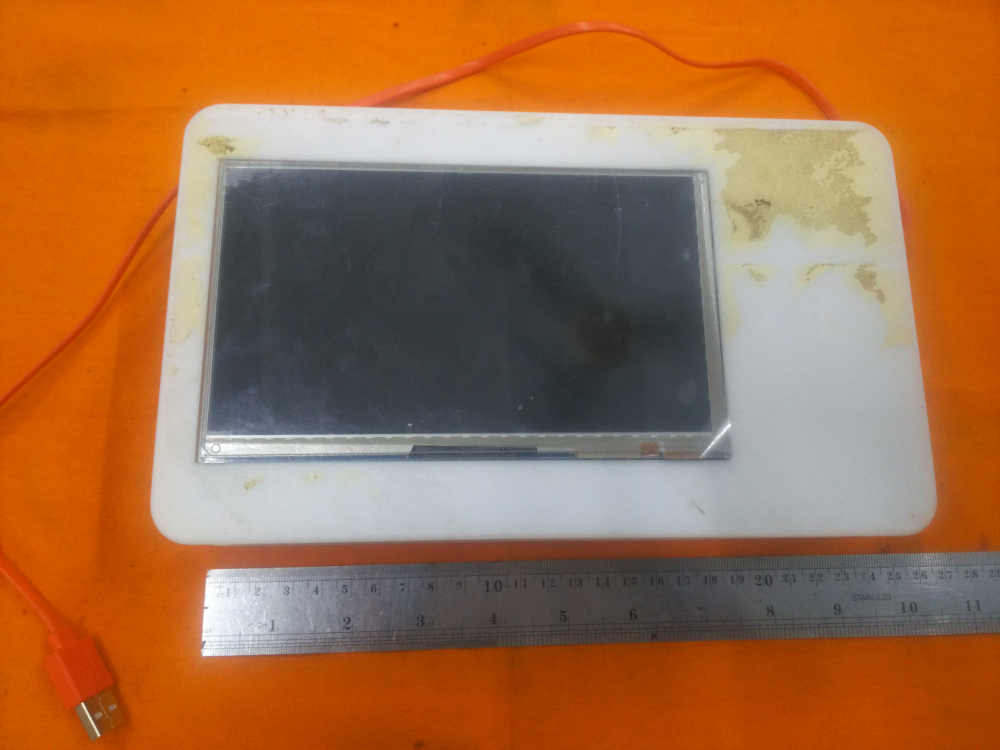
\includegraphics[width=0.25\textwidth]{images/photos/size_brin}} &
				\begin{itemize}[topsep=0pt]
					\item Cukup Besar
					\item Perlu di atas meja
				\end{itemize} &
				\raisebox{-\totalheight}{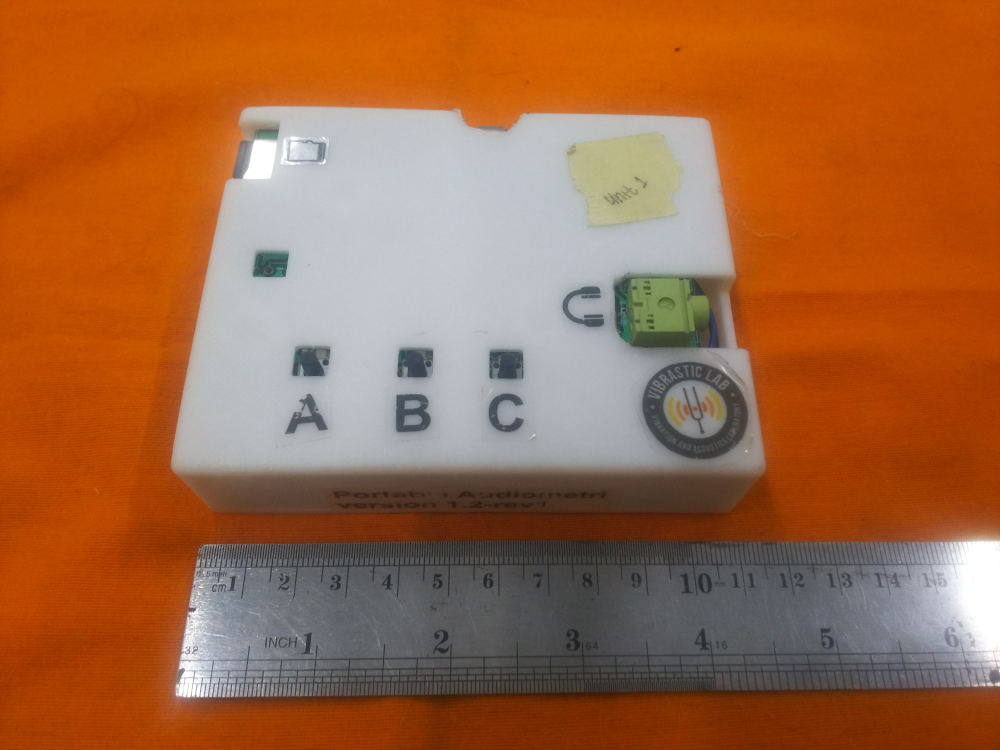
\includegraphics[width=0.25\textwidth]{images/photos/size_lpdp}} &
				\begin{itemize}[topsep=0pt]
					\item Handheld
					\item Bisa dipegang tanpa meja
				\end{itemize}
				\\ \midrule
				
				\textit{System Core} &
				\raisebox{-\totalheight}{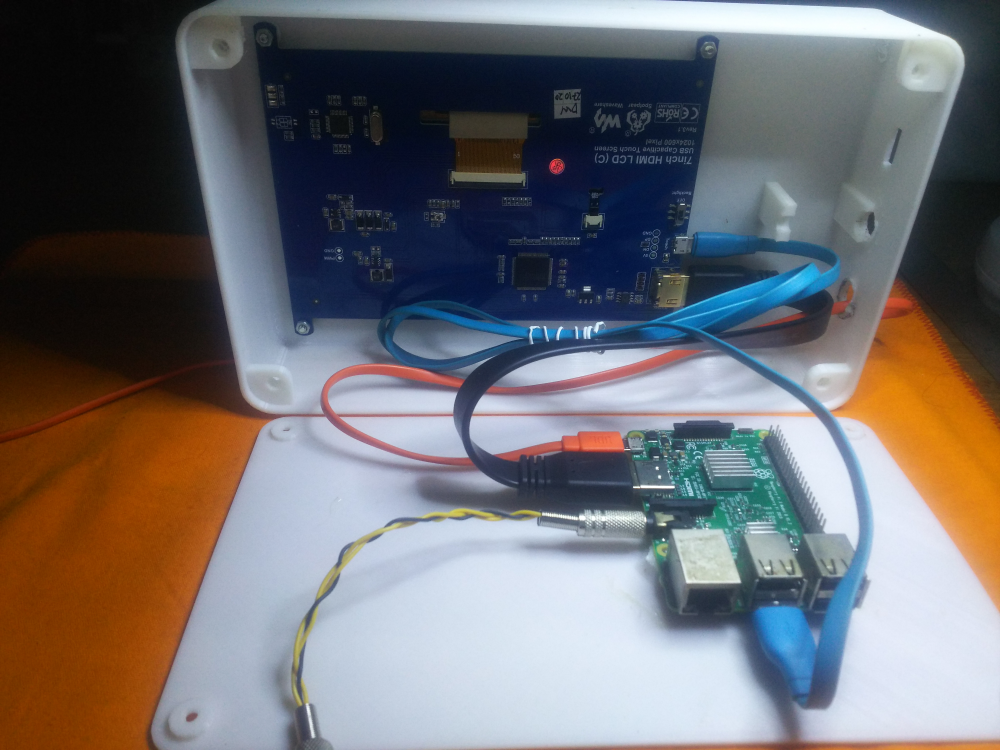
\includegraphics[width=0.25\textwidth]{images/photos/core_brin}} &
				\begin{itemize}[topsep=0pt]
					\item Berbasis Raspberry-Pi
					\item Berorientasi sebagai \textit{Mini-Computer}
				\end{itemize} &
				\raisebox{-\totalheight}{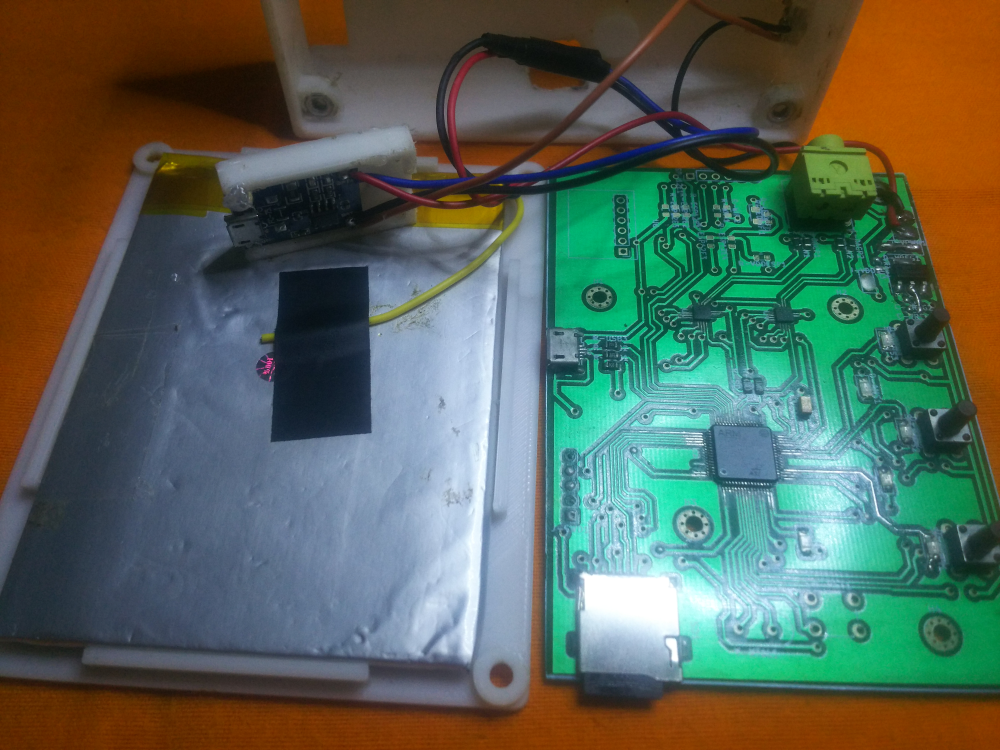
\includegraphics[width=0.25\textwidth]{images/photos/core_lpdp}} &
				\begin{itemize}[topsep=0pt]
					\item Berbasis STM32F4
					\item Berorientasi sebagai \textit{Embedded System}
				\end{itemize}
				\\ \midrule
				
				Sumber Daya &
				\raisebox{-\totalheight}{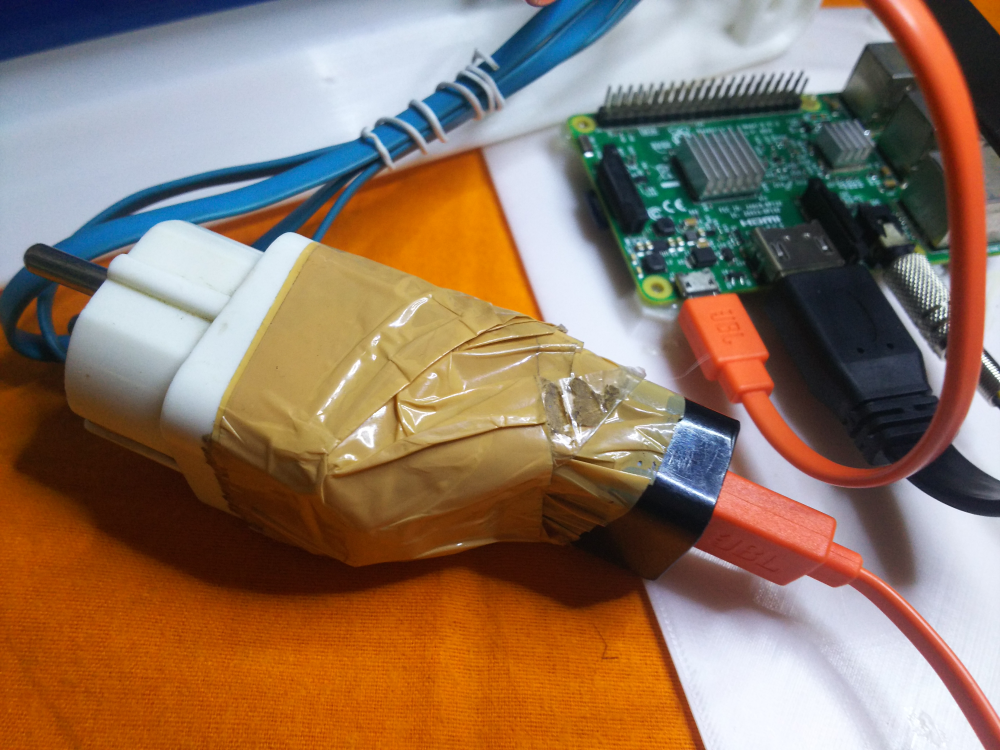
\includegraphics[width=0.25\textwidth]{images/photos/pwr_brin}} &
				\begin{itemize}[topsep=0pt]
					\item 5v-USB Adaptor (min. 1.5A) 
					\item Tidak ada battery
					\item \textit{Core chip} Raspberry dan layar sentuh membutuhkan daya besar
				\end{itemize} &
				\raisebox{-\totalheight}{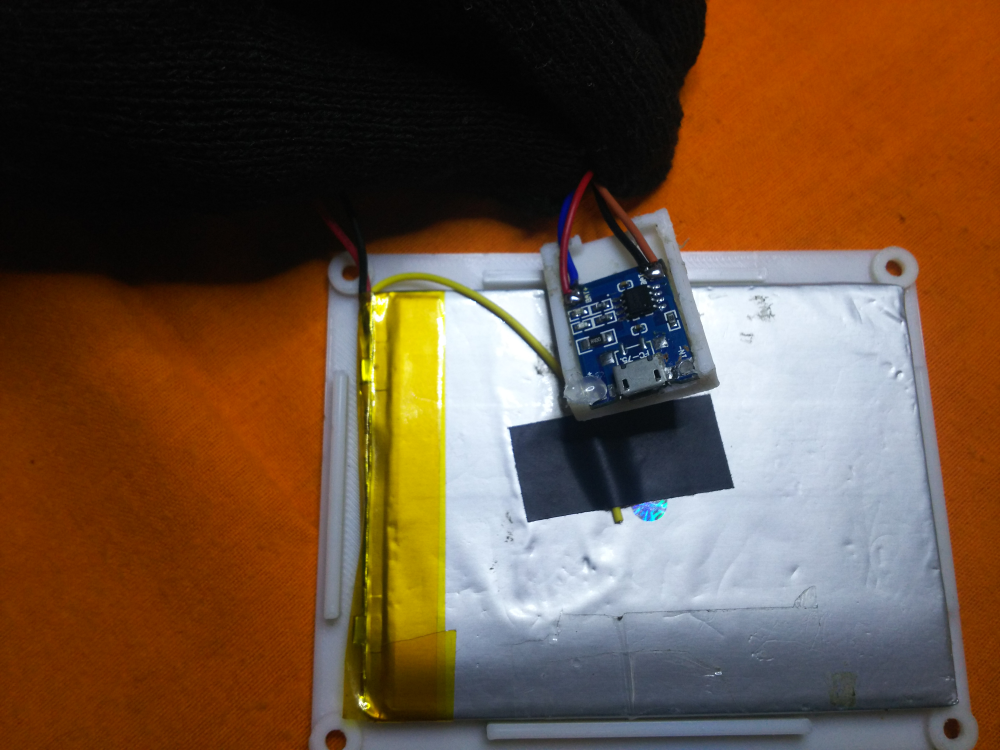
\includegraphics[width=0.25\textwidth]{images/photos/pwr_lpdp}} &
				\begin{itemize}[topsep=0pt]
					\item Battery LiPO single-cell (3.7v) 
					\item Dilengkapi \textit{charging-manager} TC4056
					\item Konsumsi daya signifikan hanya chip utama STM32F4
				\end{itemize}
				\\
				
				\bottomrule
			\end{tabular}
			\end{center}
	\end{table}

		%%%%%%%%%%%%%%%%%%%%%%%%%%%%%%%%%%%%%%%%%%%%%%%%%%%%%%%%%%%%%%%%%
	
	\newpage
	\begin{table}[h!]
		\begin{center}
			\begin{tabular}{|p{3cm}|c|p{4cm}|c|p{4cm}|}
				\toprule
				Topik & BRIN & Keterangan & RISPRO & Keterangan \\ 
				\midrule
				
				\textit{Operating System} &
				\raisebox{-\totalheight}{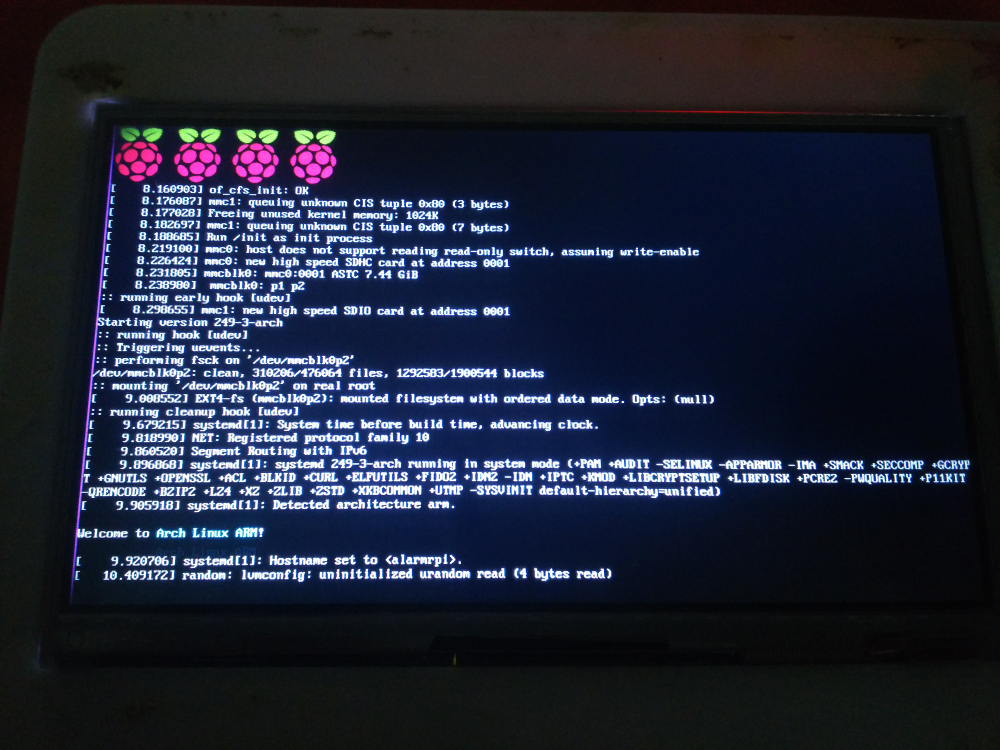
\includegraphics[width=0.25\textwidth]{images/photos/os_brin}} &
				\begin{itemize}[topsep=0pt]
					\item Mengunakan Linux armhf
					\item \textit{Booting time} berkisar 2-5 menit
					\item Tidak ada \textit{checking routine}
				\end{itemize} &
				\raisebox{-\totalheight}{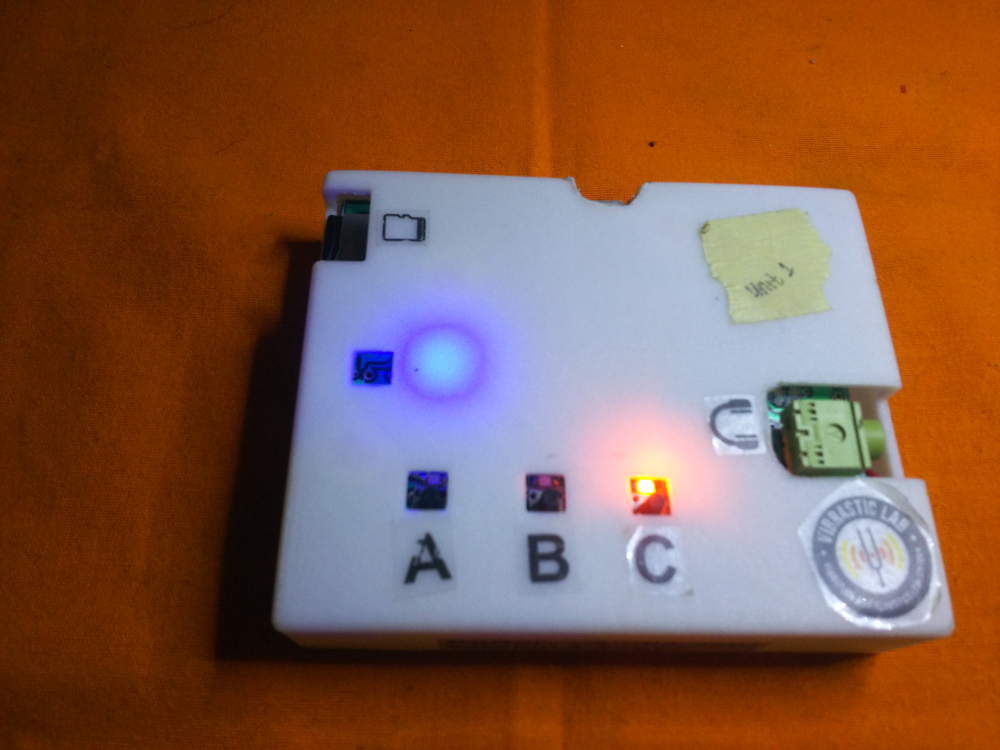
\includegraphics[width=0.25\textwidth]{images/photos/os_lpdp}} &
				\begin{itemize}[topsep=0pt]
					\item Mengunakan ChibiOS/RT (Real-Time OS)
					\item Tidak ada \textit{booting-time}
					\item \textit{Checking routine} hanya 5 detik
				\end{itemize}
				\\ \midrule
				
				\textit{Default Usage} &
				\raisebox{-\totalheight}{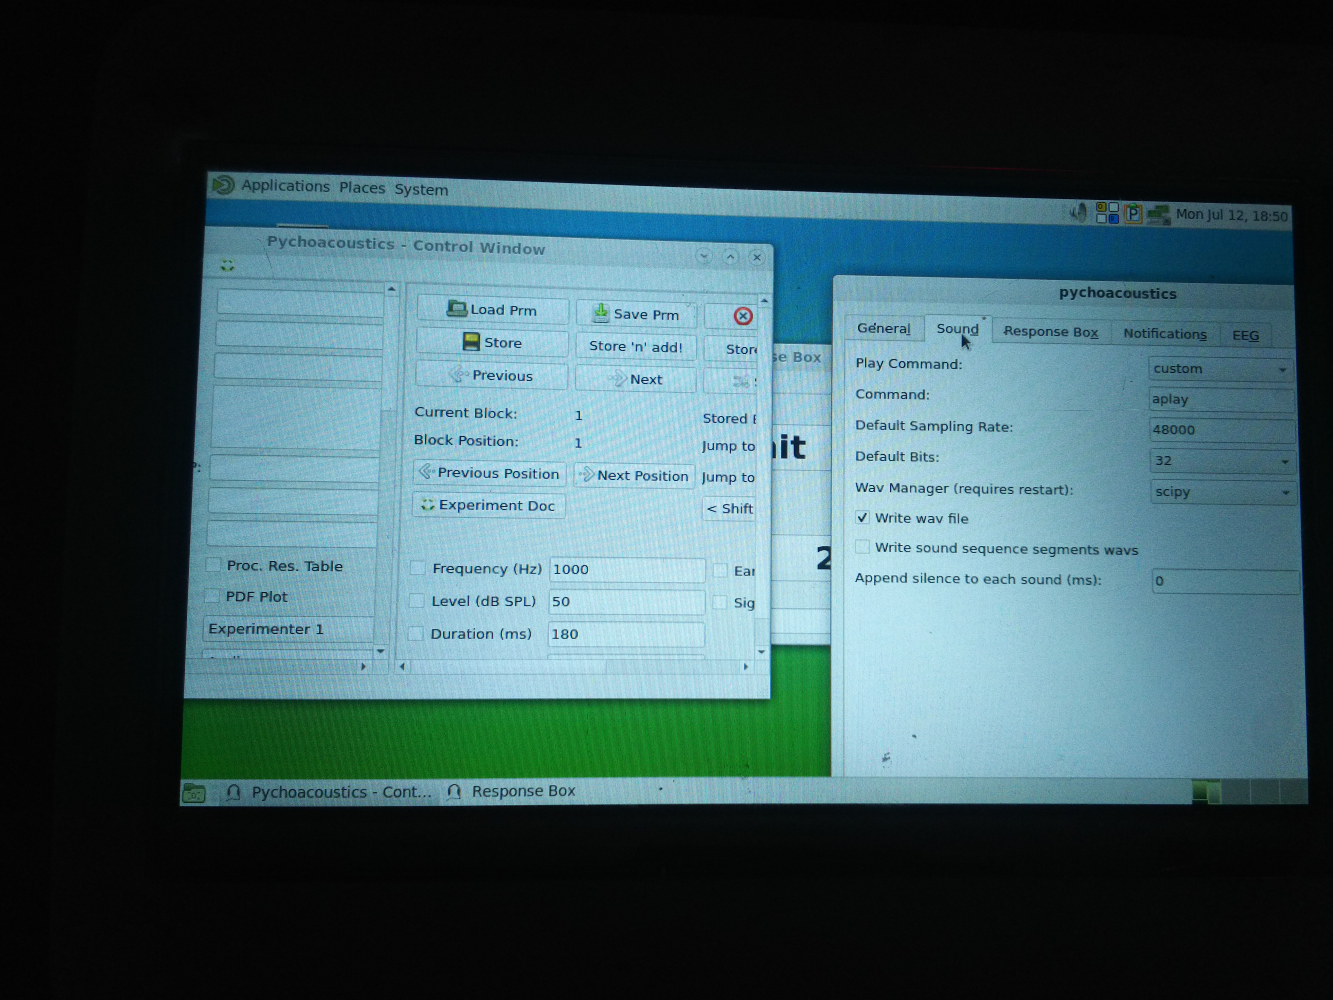
\includegraphics[width=0.25\textwidth]{images/photos/use_brin}} &
				\begin{itemize}[topsep=0pt]
					\item Membutuhkan pengaturan sebelum digunakan
					\item Tidak ada default saat program \textit{fresh-install}
				\end{itemize} &
				\raisebox{-\totalheight}{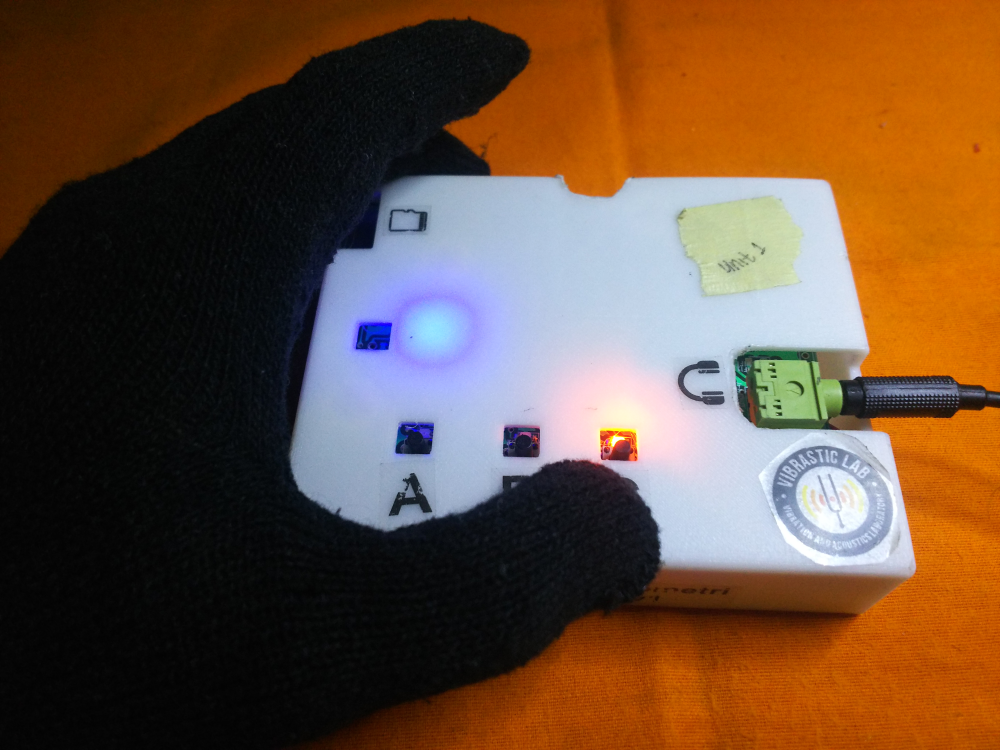
\includegraphics[width=0.25\textwidth]{images/photos/use_lpdp}} &
				\begin{itemize}[topsep=0pt]
					\item Pengaturan sudah disiapkan internal
					\item Dapat langsung digunakan secara default
				\end{itemize}
				\\ \midrule
				
				\textit{Blueprint} &
				\raisebox{-\totalheight}{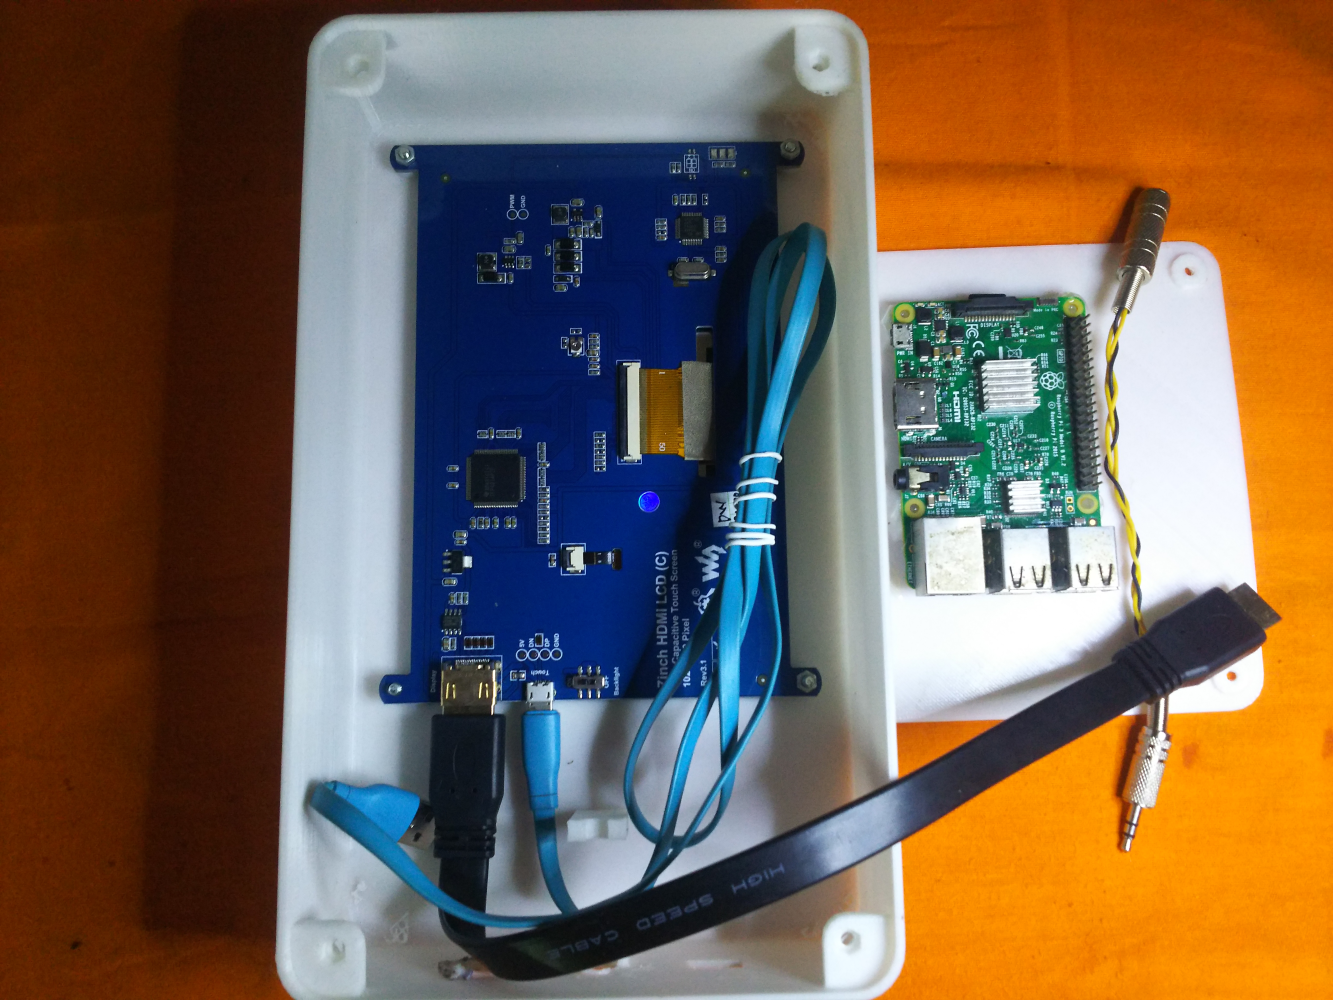
\includegraphics[width=0.25\textwidth]{images/photos/tech_brin}} &
				\begin{itemize}[topsep=0pt]
					\item Komponen modular buatan vendor lain
					\item Blueprint modul kembali kepada vendor RaspberryPi dan Waveshare
				\end{itemize} &
				\raisebox{-\totalheight}{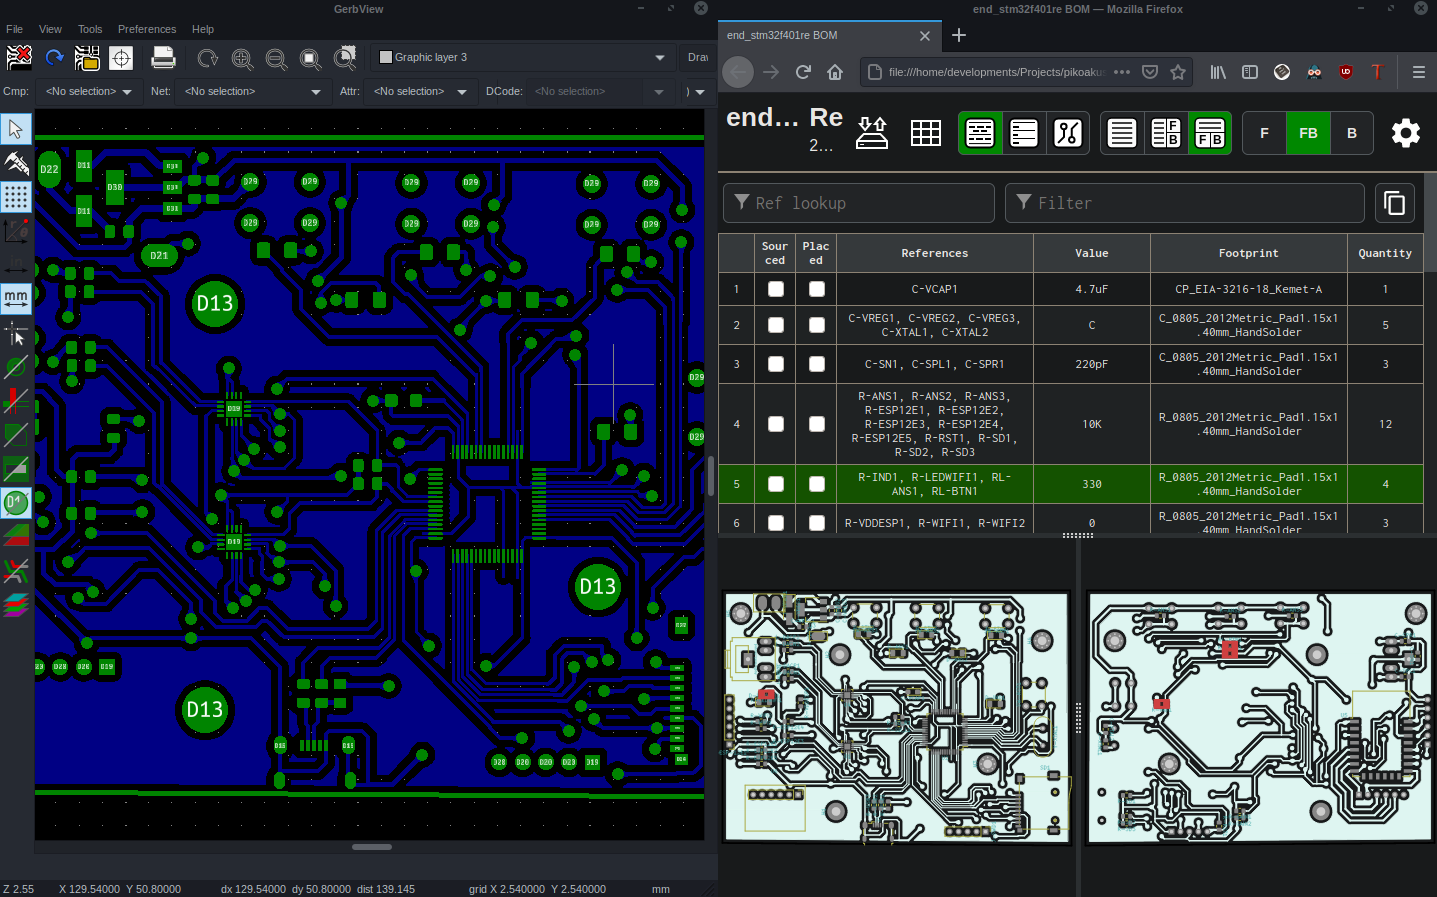
\includegraphics[width=0.25\textwidth]{images/photos/tech_lpdp}} &
				\begin{itemize}[topsep=0pt]
					\item Standar file Gerber dan BoM siap dikirim ke fabrikasi elektronik
					\item Blueprint dapat direview di \href{https://github.com/VibrasticLab/pikoakustik/tree/stm32f401re_3pin/circuit/test_3rev1/fabricate_PCB}{tautan ini}.
				\end{itemize}
				\\ \midrule
				
				\bottomrule
			\end{tabular}
		\end{center}
	\end{table}
\end{document}